\documentclass[12pt]{article}

\usepackage{sbc-template}

\usepackage{graphicx,url}

\usepackage{algorithm}
\usepackage{algpseudocode}

\usepackage{amssymb}
\usepackage{mathtools}

%\usepackage[brazil]{babel}   
\usepackage[latin1]{inputenc}  
     
\sloppy

\title{UKP5: a New Algorithm for the Unbounded Knapsack Problem}

\author{Henrique Becker \and Luciana S. Buriol}

\address{Instituto de Inform�tica -- Universidade Federal do Rio Grande do Sul
  (UFRGS)\\
  Caixa Postal 15.064 -- 91.501-970 -- Porto Alegre -- RS -- Brazil
  \email{\{hbecker,buriol\}@inf.ufrgs.br}
}

\begin{document} 

\maketitle

\begin{abstract}
In this extended abstract % resumo extendido -- short paper?
we present UKP5, an algorithm for solving the unbounded knapsack problem. 
UKP5 is based on dynamic programming, but implemented in a non traditional way: instead of looking backward for stored values of subproblems, it stores incremental lower bounds forward. 
%UKP5 uses sparsity, periodicity, and dominance for speeding up computation. 
UKP5 is considerably simpler than EDUK2, the state-of-the-art algorithm for solving the problem. 
%Moreover, it can be naturally implemented using the imperative paradigm, differently from EDUK2. 
We run UKP5 and EDUK2 on a benchmark of 4540 hard instances proposed by the authors of EDUK2. 
The results reveal that UKP5 outperforms EDUK2, being 47 times faster on the average.
\end{abstract}

\begin{resumo}
Nesse resumo extendido n�s apresentamos o UKP5, um algoritmo para solucionar o \emph{unbounded knapsack problem} (problema da mochila com repeti��es).
O UKP5 � baseado em programa��o din�mica, mas implementado de uma forma n�o-tradicional: ao inv�s de olhar para tr�s para usar solu��es de subproblemas previamente computados, ele armazena limites inferiores a frente.
%UKP5 uses sparsity, periodicity, and dominance for speeding up computation. 
O UKP5 � consideravelmente mais simples que o EDUK2, o algoritmo do estado da arte para solucionar o problema.
%Moreover, it can be naturally implemented using the imperative paradigm, differently from EDUK2. 
N�s executamos o UKP5 e o EDUK2 em uma bateria de testes contendo 4540 inst�ncias consideradas dif�ceis pelos autores do EDUK2.
Os resultados mostram que o UKP5 �, em m�dia, 47 vezes mais r�pido que o EDUK2.
\end{resumo}

\section{Introduction}

The unbounded knapsack problem (UKP) is a simpler variation of the well-known bounded knapsack problem (BKP).
UKP allows the allocation of an unbounded quantity of each item type.
The UKP is NP-Hard, and thus has no known polynomial-time algorithm for solving it. 
However, it can be solved by a pseudo-polynomial dynamic programming algorithm.

Two techniques are often used for solving UKP: dynamic programming (DP) \cite{eduk}, \cite[p. 214]{gar72}, \cite[p. 311]{tchu} and branch and bound (B\&B) \cite{mtu2}. 
The state-of-the-art solver for the UKP, introduced by~\cite{pya}, is a hybrid solver that combines DP and B\&B. 
The solver's name is PYAsUKP, and it is an implementation of the EDUK2 algorithm.

\subsection{UKP Formal Notation}

An UKP instance is composed by a capacity \(c\), and a list of \(n\) items.
Each item can be referenced by its index in the item list \(i \in \{1\dots n\}\). 
Each item \(i\) has a weight value \(w_i\), and a profit value \(p_i\).
A solution is an item multiset, i.e, a set that allows multiple copies of the same element.
The sum of the items weight, or profit, of a solution \(s\) is denoted by \(w_s\), or \(p_s\).
A valid solution \(s\) has \(w_s \leq c\).
An optimal solution \(s^*\) is a valid solution with the greatest profit among all valid solutions.
The UKP objective is to find an optimal solution for the given UKP instance. 
The mathematical formulation of UKP is:

\begin{align}
  maximize &\sum_{i=1}^n p_i x_i\label{eq:objfun}\\
subject~to &\sum_{i=1}^n w_i x_i \leq c\label{eq:capcons}\\
            &x_i \in \mathbb{N}_0\label{eq:x_integer}
\end{align}

The quantities of each item \(i\) in an optimal solution are denoted by \(x_i\), and are restricted to the non-negative integers, as~\eqref{eq:x_integer} indicates. 
%We assume that the capacity \(c\), the quantity of items \(n\) and the weights of the items \(w_i\) are positive integers. 
%The profits of the items \(p_i\) are positive real numbers.

The efficiency of an item \(i\) is the ratio \(\frac{p_i}{w_i}\), and is denoted by \(e_i\). 
We use \(w_{min}\) and \(w_{max}\) to denote the smallest item weight, and the biggest item weight, respectively. 
Also, we refer to the item with the lowest weight among the ones tied with the greatest efficiency as the \emph{best item}, % CHECAR SE NECESS�RIO
and the item with the lowest weight among all items as the \emph{smallest item}. % CHECAR SE NECESS�RIO

\section{UKP5: The Proposed Algorithm}

UKP5 is inspired by the DP algorithm described by Garfinkel~\cite[p. 221]{gar72}. 
The name ``UKP5'' is due to five improvements applied over that algorithm: \textbf{Symmetry pruning}: symmetric solutions are pruned in a more efficient fashion than in~\cite{gar72};
\textbf{Sparsity}: not every position of the optimal solutions value array has to be computed;
\textbf{Dominated solutions pruning}: dominated solutions are pruned;
\textbf{Time/memory tradeoff}: the test \(w_i \leq y\) from the algorithm in~~\cite{gar72} was removed in cost of more O(\(w_{max}\)) memory;
\textbf{Periodicity}: the periodicity check suggested in~\cite{gar72} (but not implemented there) was adapted and implemented.

\begin{algorithm}[!t]
\caption{UKP5 -- Computation of $opt$}\label{alg:ukp5}
\begin{algorithmic}[1]
\Procedure{UKP5}{$n, c, w, p, w_{min}, w_{max}$}
  \State \(g \gets\) array of \(c + w_{max}\) positions each one initialized with \(0\)\label{create_g}
  \State \(d \gets\) array of \(c + w_{max}\) positions each one initialized with \(n\)\label{create_d}
  
  \For{\(i \gets 1, n\)}\label{begin_trivial_bounds}\Comment{Stores one-item solutions}
    \If{\(g[w_i] < p_i\)}
      \State \(g[w_i] \gets p_i\)
      \State \(d[w_i] \gets i\)
    \EndIf
  \EndFor\label{end_trivial_bounds}

  \State \(opt \gets 0\)\label{init_opt}

  \For{\(y \gets w_{min}, c\)}\label{main_ext_loop_begin}\Comment{Can end early because of periodicity check}
    \If{\(g[y] \leq opt\)}\label{if_less_than_opt_begin}\Comment{Handles sparsity and pruning of dominated solutions}
    	\State \textbf{continue}\label{alg:continue}\Comment{Ends current iteration and begins the next}
    \EndIf\label{if_less_than_opt_end}
    
    \State \(opt \gets g[y]\)\label{update_opt}
    
    \For{\(i=1,d[y]\)}\label{main_inner_loop_begin}\Comment{Creates new solutions (never symmetric)}
      \If{\(g[y + w_i] < g[y] + p_i\)}\label{if_new_lower_bound_begin}
        \State \(g[y + w_i] \gets g[y] + p_i\)
        \State \(d[y + w_i] \gets i\)
%      \ElsIf{\(g[y + w_i] = g[y] + p_i \land i < d[y + w_i]\)}
%        \State \(d[y + w_i] \gets i\)
      \EndIf\label{if_new_lower_bound_end}
    \EndFor\label{main_inner_loop_end}
  \EndFor\label{main_ext_loop_end}
  \State \textbf{return} \(opt\)

%  \For{\(y \gets c-w_{min}+1, c\)}\label{get_y_opt_loop_begin}\Comment{Removal of dominated solutions}
%    \If{\(g[y] > opt\)}\label{last_loop_inner_if}
%      \State \(opt \gets g[y]\)
%      \State \(y_{opt} \gets y\)
%    \EndIf
%  \EndFor\label{get_y_opt_loop_end}
\EndProcedure
\end{algorithmic}
\end{algorithm}

With the intent of making easier to the reader to undestand the core ideia of the UKP5 algorithm, the pseudocode presented at Algorithm \ref{alg:ukp5} was stripped of many optimizations. Some of them are: all the items are sorted by non-increasing efficiency and, between items with the same efficiency, by increasing weight; the \(y^{*}\) periodicity bound is computed as in~\cite[p. 223]{gar72}, and used to reduce the \(c\) value; we make use of a UKP5-specific periodicity check described below.

Our periodicity check is a stopping condition inside UKP5 main loop (\ref{main_ext_loop_begin} and \ref{main_ext_loop_end}). 
Let \(y\) be the value of the variable \(y\) at line \ref{main_ext_loop_begin}, and let \(y'\) be the biggest capacity where \(g[y'] \neq 0 \land d[y'] > 1\). 
If at some moment \(y > y'\) then we can stop the computation and fill the remaining capacity with copies of the first item (item of index \(1\)).
This periodicity check works only if the first item is the best item. 
If this assumption is false, then the described condition will never happen, and the algorithm will iterate until \(y = c\) as usual.

\section{Computational Results and Analysis}

\begin{figure}[th]
  \label{fig:times}
  \centering
  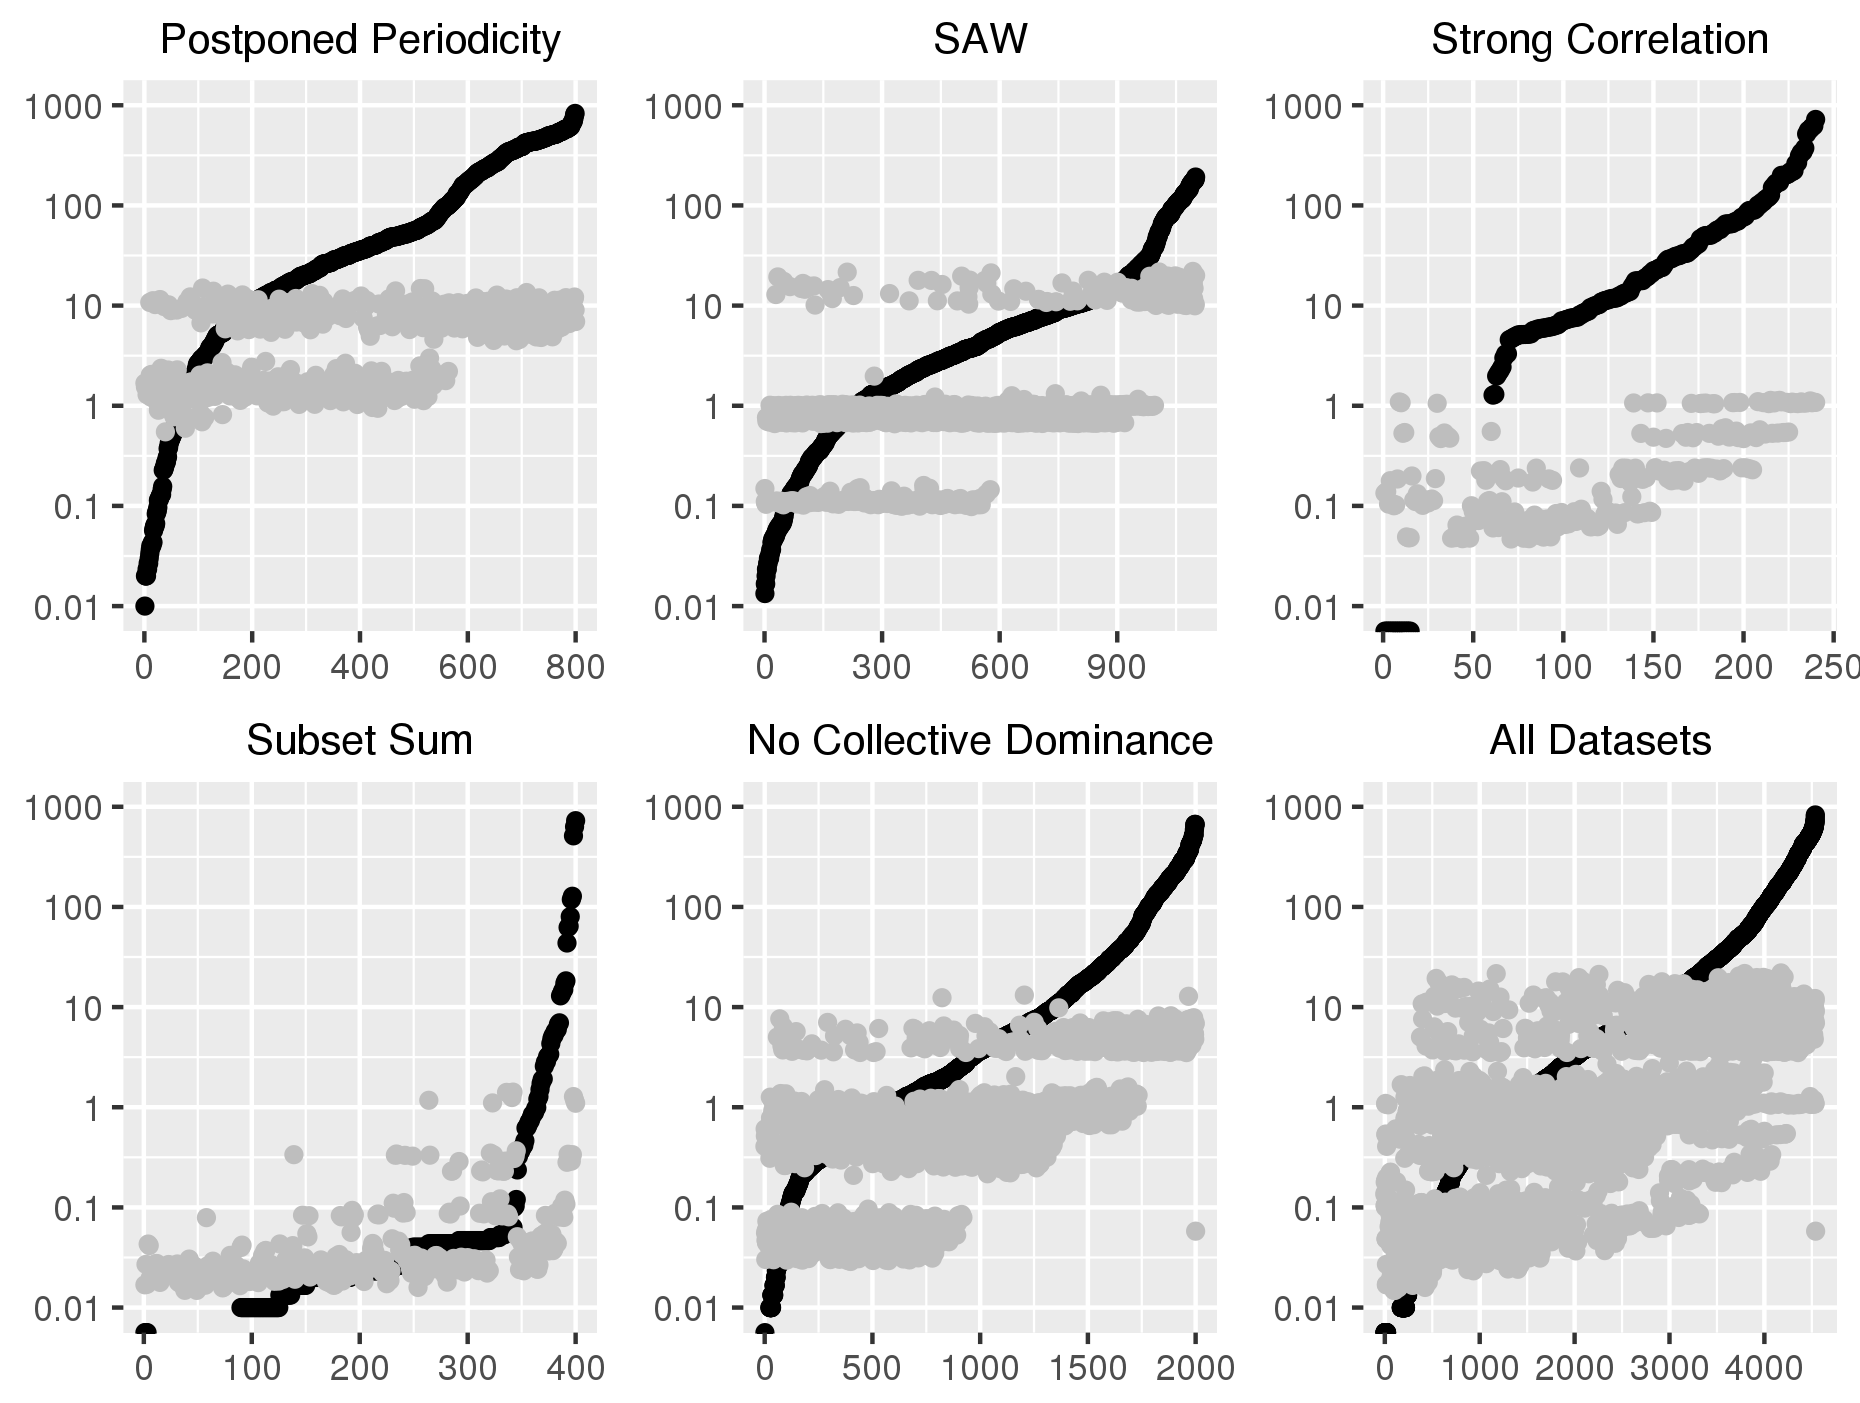
\includegraphics[width=\textwidth]{six_plots.png}
  \caption{The times used by UKP5 and PYAsUKP for each instance of each class. The black dots represent PYAsUKP times. The gray dots represent UKP5 times. The y axis is the time used to solve an UKP instance, in seconds. The x axis is the instance index when the instances are are sorted by the time PYAsUKP took to solve it. Note that the y axis is in logarithmic scale.}
\end{figure}

\section{Conclusion and Final Remarks}


\bibliographystyle{sbc}
\bibliography{sbc-template}

\end{document}
